% Chapter 1

\chapter{Organisation de l'équipe et planning} % Main chapter title

\label{Chapter1} % For referencing the chapter elsewhere, use \ref{Chapter1}

%----------------------------------------------------------------------------------------

\section{Organisation de l'équipe}

Après notre entrevue, nous avons décidé de nous séparer en deux groupes un qui
partirait du haut niveau et un autre qui partirait du bas niveau. Le but de
cette méthode est de pouvoir mieux appréhender les différents problèmes et axes
de développement. Le binôme Clément \& Romain recherche à faire le lien depuis
les couches applicatives vers le kernel. Le binôme Alan \& Martin au contraire
cherche à établir en priorité les couches basses pour ensuite les rendre
compatible avec le kernel. Pour résumer les deux binômes n’ont pas le même point
de départ tout en ayant la même version du kernel.

Clément et Romain sont donc chargés de l’utilisation de Gstreamer et de la
couche V4L alors que Martin et Alan sont chargés de rendre les drivers
compatibles avec notre système.

\section{Planning}

Nous vous avons ici présenté un planning des taches effectuer durant ces 8 \\
derniers jours, les noms attribués à chaque tache seront développées dans la suite du rapport.

\begin{figure}[th]
    \centering
    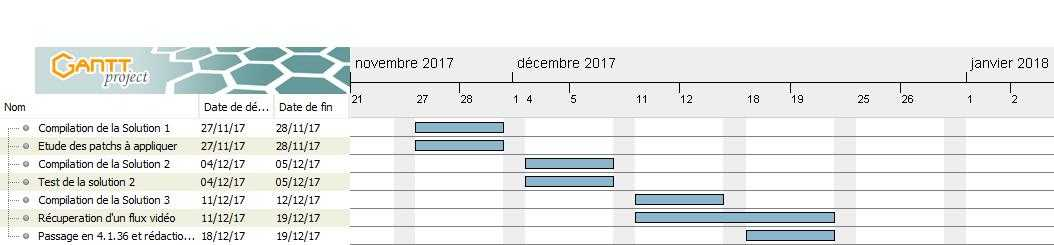
\includegraphics[width=1\linewidth]{planning.png}
    \decoRule
    \caption{Avancement du projet actuel}  \label{fig:planning}
\end{figure}

Les trois solutions qui sont présentées ci-dessous correspondent à trois codes sources.

%----------------------------------------------------------------------------------------
